\documentclass[mathserif]{beamer}
\usepackage[utf8]{inputenc}

% packages
\usepackage{physics}
\usepackage{amsfonts, amsmath, amssymb, amsthm}
\usepackage{systeme}
\usepackage[none]{hyphenat}
\usepackage{fancyhdr}
\usepackage{graphicx}
\graphicspath{{./images/}}
\usepackage{float}
\usepackage{siunitx}
\usepackage{esint}
\usepackage{cancel}
\usepackage{mathtools}

% colors
\usepackage{xcolor}
\definecolor{p}{HTML}{FFDDDD}
\definecolor{g}{HTML}{D9FFDF}
\definecolor{y}{HTML}{FFFFCF}
\definecolor{b}{HTML}{D9FFFF}
\definecolor{o}{HTML}{FADECB}
%\definecolor{}{HTML}{}

% \highlight[<color>]{<stuff>}
\newcommand{\highlight}[2][p]{\mathchoice%
  {\colorbox{#1}{$\displaystyle#2$}}%
  {\colorbox{#1}{$\textstyle#2$}}%
  {\colorbox{#1}{$\scriptstyle#2$}}%
  {\colorbox{#1}{$\scriptscriptstyle#2$}}}%

% paragraph indentation/spacing
\setlength{\parindent}{0cm}
\setlength{\parskip}{5pt}
\renewcommand{\baselinestretch}{1.25}

\newcommand{\br}[1]{\left(#1\right)}
\newcommand{\sbr}[1]{\left[#1\right]}
\newcommand{\cbr}[1]{\left\{#1\right\}}

\usetheme{Madrid}
\usecolortheme{default}

%------------------------------------------------------------
%This block of code defines the information to appear in the title page
\title[The inverse Laplace transform] %optional
{The inverse Laplace transform}

\subtitle{via the Bromwich integral}

\author[Sai Sivakumar] % (optional)
{Sai Sivakumar}

\AtBeginSection[]{
  \begin{frame}
  \vfill
  \centering
  \begin{beamercolorbox}[sep=8pt,center,shadow=true,rounded=true]{title}
    \usebeamerfont{title}\insertsectionhead\par%
  \end{beamercolorbox}
  \vfill
  \end{frame}
}

\begin{document}

%The next statement creates the title page.
\frame{\titlepage}

%This block of code is for the table of contents after the title page
\begin{frame}
\frametitle{outline}
\tableofcontents
\end{frame}

\section{the Laplace transform}

\begin{frame}
  \frametitle{brief summary}

  \begin{theorem}[Laplace transform]
    Let $F(t)$ be sectionally continuous on every finite interval $0\leq t\leq T$ and also of exponential order, so that $\abs{F(t)}\in O(e^{at})$ where $t\geq 0$.

    Then for complex $s$ the Laplace transform of $F(t)$ is \[f(s) = \int_0^\infty e^{-st}F(t)\dd{t}\] and is analytic in the half plane where $\Re(s) > a$
  \end{theorem}

  % note meanings of sectionally continuous and exponential order, also note uses
\end{frame}

\begin{frame}
  \frametitle{properties of the transform}

  Linearity: $\mathcal{L}[f(t)+g(t)] = \mathcal{L}[f(t)] + \mathcal{L}[g(t)]$

  Time shift: $\mathcal{L}[f(t-a)u(t-a)] = e^{-as}\mathcal{L}[f(t)]$, $a\geq 0$

  Complex shift: $\mathcal{L}[e^{at}f(t)](s) = \mathcal{L}[f(t)](s-a)$

  Transform of the $n$-th derivative: $\mathcal{L}[f^{(n)}(t)](s) = s^n\mathcal{L}[f(t)](s) - s^{n-1}f(0) - s^{n-2}f^{\prime}(0) - \cdots - f^{(n-1)}(0)$

  Convolution: $\mathcal{L}[(f\ast g)(t)] = \mathcal{L}[f(t)]\mathcal{L}[g(t)]$
  
\end{frame}

\begin{frame}
  \frametitle{non-unique inverses?}

  If two functions agree everywhere except at countably many points, their Laplace transforms will be the same.

  Furthermore, if two continuous functions have the same Laplace transform, then they must be the same function.

  %There is a way to do it, but it's kind of complicated so I will not show this here. 
  
  See Lerch's theorem for more.

\end{frame}

\section{the inversion problem}

\begin{frame}
  \frametitle{using a table?}

  \begin{columns}

    \column{0.3\textwidth}
    I guess so...
    \column{0.5\textwidth}
    \begin{figure}[h]
      \centering
      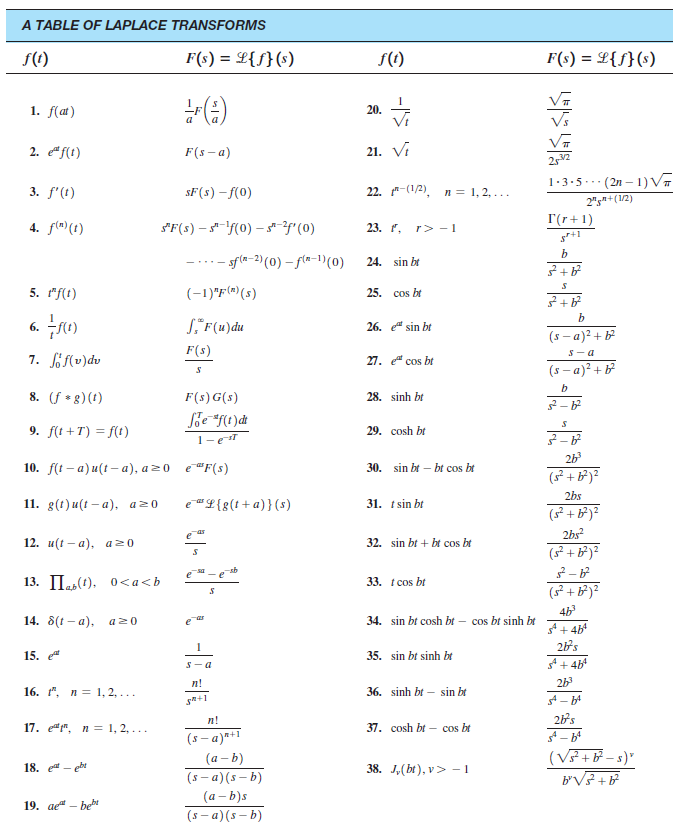
\includegraphics[scale=0.33]{table}
    \end{figure}
  \end{columns}

\end{frame}

\begin{frame}
  \frametitle{handwavey motivation}

  We can start by extending Cauchy's integral formula for a specific class of functions.

  Recall that Cauchy's integral formula gives you the value of an analytic function $f$ at a point $z_0$ inside a simple closed contour $C$ by the following: \[f(z_0) = \frac{1}{2\pi i}\int_C \frac{f(z)}{z-z_0}\dd{z}\]

\end{frame}

\begin{frame}
  \frametitle{extending Cauchy's integral formula}

  \begin{theorem}[Cauchy integral formula extension]
    Let $f(z)$ be analytic where $\Re(z) \geq \gamma$ and also be of order $O(z^{-k})$, where $\gamma, k$ are real and $k> 0$. 
    
    Then if $z_0$ is a complex number where $\Re(z_0) > \gamma$, \[f(z_0) = -\frac{1}{2\pi i}\int_{\gamma-i\infty}^{\gamma + i\infty}\frac{f(z)}{z-z_0}\dd{z}.\]
  \end{theorem}

  % principal value comment

\end{frame}

\begin{frame}
  \frametitle{proof}

  % rectangular contour
  \begin{columns}

    \column{0.47\textwidth}
    Construct the contour $S$:
    \column{0.5\textwidth}
    \begin{figure}[h]
      \centering
      
\includegraphics[scale=0.25]{1}
    \end{figure}
  \end{columns}

  Apply Cauchy's integral formula to find \[f(z_0) = \frac{1}{2\pi i}\sbr{-\int_{\gamma-i\beta}^{\gamma + i\beta}\frac{f(z)}{z-z_0}\dd{z} + \int_S\frac{f(z)}{z-z_0}\dd{z}}.\] 

  % second integral needs to vanish, draw picture

\end{frame}

\begin{frame}
  \frametitle{proof}

  To show that the second integral vanishes as $\beta$ goes to infinity, use a bounding argument. % ML inequality
  
  From the order condition imposed on $f(z)$, it follows that \[\abs{\frac{f(z)}{z-z_0}} \leq \frac{M}{\abs{z}^k\abs{z-z_0}} = \frac{M}{\abs{z}^{k+1}\abs{1-(z_0/z)}},\] where $M$ is the maximum value of $f(z)$ on $S$.

\end{frame}

\begin{frame}
  \frametitle{proof}

  Note that $\abs{z}\geq \beta$, since $z\in S$.
  
  If we take $\beta$ to be large enough, say $\beta > 2\abs{z_0}$, so that $\abs{z_0} < \abs{z}/2$ or otherwise $\abs{z_0/z} < 1/2$, then by the reverse triangle inequality (or otherwise) see that \[\abs{1-(z_0/z)}\geq \abs{\abs{1}-\abs{z_0/z}} > 1-\abs{z_0/z} > 1/2.\]

  % start from \abs{1} and add and subtract z_0/z and apply triangle inequality for alternate method

  

\end{frame}

\begin{frame}
  \frametitle{proof}

  We can then bound the integrand above, so that \[\abs{\frac{f(z)}{z-z_0}} < \frac{2M}{\abs{z}^{k+1}} \leq \frac{2M}{\br{\sqrt{2}\beta}^{k+1}} < \frac{2M}{\beta^{k+1}}.\]

  See that the length of $S$ is $\beta + \beta + (\beta-\gamma) + (\beta-\gamma) = 4\beta-2\gamma$.

\end{frame}

\begin{frame}
  \frametitle{proof}

  We can bound the second integral, so that \[\abs{\int_S\frac{f(z)}{z-z_0}\dd{z}} < \frac{2M}{\beta^{k+1}}\int_S \abs{\dd{z}} = \frac{2M}{\beta^k}\br{4-\frac{2\gamma}{\beta}}.\] Then since $k>0$, if we let $\beta$ become arbitrarily large, the second integral vanishes. 

\end{frame}

\begin{frame}
  \frametitle{proof}

  From Cauchy's integral formula we had that \[f(z_0) = \frac{1}{2\pi i}\sbr{-\int_{\gamma-i\beta}^{\gamma + i\beta}\frac{f(z)}{z-z_0}\dd{z} + \int_S\frac{f(z)}{z-z_0}\dd{z}},\] but because $\beta$ was arbitrary, we may take $\beta\to\infty$, so that \[f(z_0) = -\frac{1}{2\pi i}\int_{\gamma-i\infty}^{\gamma + i\infty}\frac{f(z)}{z-z_0}\dd{z}.\] This completes the proof.

\end{frame}

\begin{frame}
  \frametitle{handwaving begins here}

  Let $f(s)$ be analytic and of order $O(s^{-k}), k> 0$ for all points where $\Re(s)\geq \gamma$. Then from the extension to Cauchy's integral formula we have \[f(s) = -\frac{1}{2\pi i}\int_{\gamma-i\infty}^{\gamma+i\infty}\frac{f(z)}{z-s}\dd{z}, \] which we can rewrite as \[f(s) = \lim_{\beta\to \infty}\frac{1}{2\pi i}\int_{\gamma-i\beta}^{\gamma+i\beta}\br{\frac{1}{s-z}}f(z)\dd{z}.\] (holds for all $s$ such that $\Re(s) > \gamma$)

\end{frame}

\begin{frame}
  \frametitle{handwaving ends after this}

  Then apply the inverse Laplace transform \textbf{formally} to $f(s)$, we have that \[F(t) = \mathcal{L}^{-1}\sbr{f(s)} = \lim_{\beta\to \infty}\frac{1}{2\pi i}\int_{\gamma-i\beta}^{\gamma+i\beta} \mathcal{L}^{-1}\sbr{\frac{1}{s-z}}f(z)\dd{z}\] \[ = \lim_{\beta\to \infty}\frac{1}{2\pi i}\int_{\gamma-i\beta}^{\gamma+i\beta}e^{zt}f(z)\dd{z}.\]

  This does not prove anything! it is just cute

\end{frame}

\begin{frame}
  \frametitle{the inversion integral}

  % give full theorem, point out which parts will be shown/omitted/weakened

  \begin{theorem}[Laplace inversion integral]
    Let $f(s)$ ($s = x+iy$) be analytic and of order $O(s^{-k}), k > 1$ where $x \geq x_0$, and also let $f(x)$ be real valued for $x\geq x_0$.
    
    Then for any $\gamma \geq x_0$, \[F(t) = \lim_{\beta \to \infty}\frac{1}{2\pi i}\int_{\gamma - i\beta}^{\gamma + i\beta}e^{zt}f(z)\dd{z},\] where $F(t)$ is a real valued function independent of $\gamma$.

    Furthermore, the Laplace transform of $F(t)$ is indeed $f(s)$, and $F(t)$ is of order $O(e^{x_0t})$.
  \end{theorem}

  % insert integral and picture of contour

\end{frame}

\begin{frame}
  \frametitle{independence of choice of $\gamma$?}

  

  % insert image
  \begin{columns}

    \column{0.47\textwidth}
    We can pick a second path where instead of $\gamma$ we choose $\gamma^{\prime}$, where $\gamma^{\prime}> \gamma$. Form a rectangular contour like so:
    \column{0.5\textwidth}
    \begin{figure}[h]
      \centering
      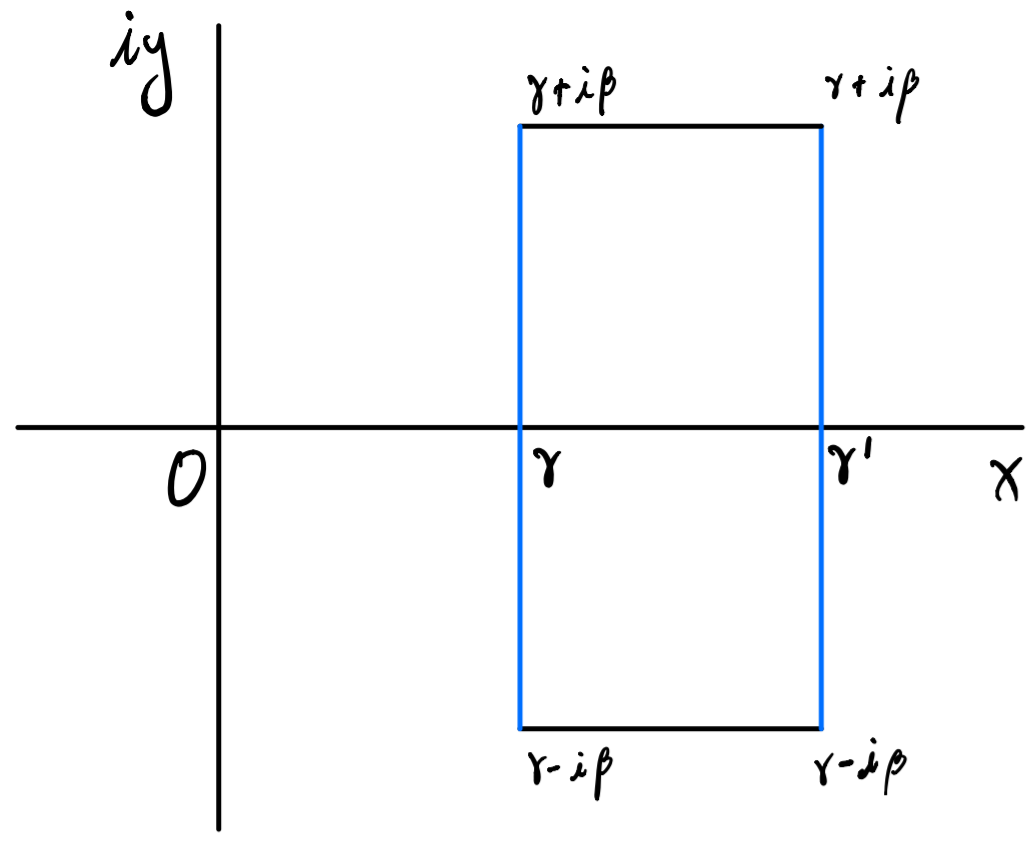
\includegraphics[scale=0.25]{2}
    \end{figure}
  \end{columns}

  Observe that the integral around the rectangle is zero since $f(s)$ is analytic on the rectangle and in it.

\end{frame}

\begin{frame}
  \frametitle{inspect the horizontal bits}

  For points on $BC$, $z = x+i\beta$ (so $\abs{z} > \beta$ if $\gamma > 0$), and from the order condition on $f(s)$ we have that \[\abs{e^{zt}f(z)}\leq e^{xt}\abs{f(z)}\leq e^{xt}\frac{M}{\abs{z}^k} < e^{xt}\frac{M}{\beta^k},\]

  and so we can bound the integral over $BC$: \[\abs{\int_{\gamma+i\beta}^{\gamma^{\prime}+i\beta}e^{zt}f(z)\dd{z}} < \frac{M}{\beta^k}\int_{\gamma}^{\gamma^{\prime}}e^{xt}\dd{x}.\]

\end{frame}

\begin{frame}
  \frametitle{the horizontal parts vanish}

  Since $\beta$ was arbitrary we may take $\beta\to \infty$, and see that the integrals over $BC$ and similarly $AD$ vanish.

  Since the integral around the rectangle was zero, we have that \[\lim_{\beta\to\infty}\sbr{\int_{\gamma-i\beta}^{\gamma+i\beta}e^{zt}f(z)\dd{z} + \int_{\gamma^{\prime}+i\beta}^{\gamma^{\prime}-i\beta}e^{zt}f(z)\dd{z}} = 0.\]

\end{frame}

\begin{frame}
  \frametitle{independence}

  So by rearranging and multiplying by $(2\pi i)^{-1}$ we have that \[\lim_{\beta\to\infty}\frac{1}{2\pi i}\int_{\gamma-i\beta}^{\gamma+i\beta}e^{zt}f(z)\dd{z} = \lim_{\beta\to\infty}\frac{1}{2\pi i}\int_{\gamma^{\prime}-i\beta}^{\gamma^{\prime}+i\beta}e^{zt}f(z)\dd{z},\] which establishes the independence of the choice of $\gamma$ in the inversion integral.

\end{frame}

\begin{frame}
  \frametitle{is this actually an inverse?}

  We wish to show that the Laplace transform of the inversion integral is equivalent to $f(s)$.

  Proceed directly. Here, choose $s\in\mathbb{C}$ such that $\Re(s)>\Re(z) = \gamma$.

  \[\mathcal{L}[F(t)] = \lim_{T\to \infty}\int_0^Te^{-st}\frac{1}{2\pi i}\int_{\gamma-i\infty}^{\gamma+i\infty}e^{zt}f(z)\dd{z}\dd{t}\]

\end{frame}

\begin{frame}
  \frametitle{integral shenanigans, mostly handwaving}

  \[\mathcal{L}[F(t)] = \lim_{T\to \infty}\int_0^Te^{-st}\frac{1}{2\pi i}\int_{\gamma-i\infty}^{\gamma+i\infty}e^{zt}f(z)\dd{z}\dd{t}\]
  \[\stackrel{?}{=}\text{ (magic)}\]
  \[\frac{1}{2\pi i}\int_{\gamma-i\infty}^{\gamma+i\infty}f(z)\lim_{T\to \infty}\int_0^T e^{(z-s)t}\dd{t}\dd{z}\]
  \[ = -\frac{1}{2\pi i}\int_{\gamma-i\infty}^{\gamma+i\infty} \frac{f(z)}{z-s}\dd{z}\]

\end{frame}

\begin{frame}
  \frametitle{something familiar}

  From the extension to Cauchy's integral formula we saw earlier, observe that \[-\frac{1}{2\pi i}\int_{\gamma-i\infty}^{\gamma+i\infty} \frac{f(z)}{z-s}\dd{z} = f(s).\]

\end{frame}

\begin{frame}
  \frametitle{using the residue theorem}

  We can use the residue theorem to evaluate the inversion integral when there are isolated singularities where $\Re(z) < \gamma$.

  Suppose $f(s)$ is a complex valued function which satisfies the conditions needed so that the inversion integral of $f(s)$ converges to $F(t)$ (whose Laplace transform is $f(s)$).

  We can also take $k\geq 1$ in the order condition, but there are lots of details.

\end{frame}

\begin{frame}
  \frametitle{the Bromwich integral}

  \begin{columns}
  \column{0.47\textwidth}
  Observe that the inversion integral is the integral over the straight part.
  \column{0.5\textwidth}
    \begin{figure}[h]
      \centering
      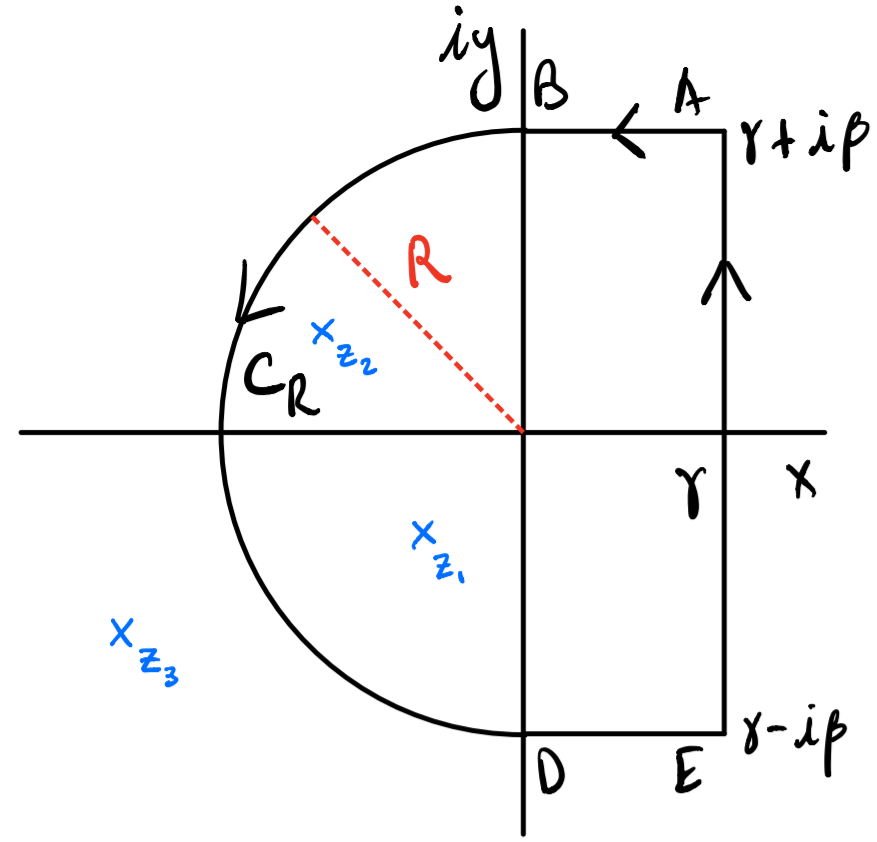
\includegraphics[scale=0.25]{3}
    \end{figure}
  \end{columns}

  We take the integral over the whole contour and show that integrals over the other segments vanish as $R$ or $\beta$ become arbitrarily large.

\end{frame}

\begin{frame}
  \frametitle{contour surgery}

  So by the residue theorem \begin{multline*}
    \int_{\gamma-i\infty}^{\gamma+i\infty} e^{zt}f(z)\dd{z} + \int_{AB} e^{zt}f(z)\dd{z} + \int_{C_R} e^{zt}f(z)\dd{z}\\ + \int_{DE} e^{zt}f(z)\dd{z} = 2\pi i\sum_k \Res(e^{zt}f(z), z_k).
  \end{multline*}

\end{frame}

\begin{frame}
  \frametitle{the horizontal bits vanish}

  See that the integral over $AB$ vanishes (the integral over $DE$ vanishes similarly).

  Here, $z=x+i\beta$, so $\abs{z}\geq\beta$. Then

  \[\abs{e^{zt}f(z)} \leq e^{xt}\abs{f(z)}\leq e^{xt}\frac{M}{\abs{z}^k} \leq e^{xt}\frac{M}{\beta^k},\] so \[\abs{\int_{AB} e^{zt}f(z)\dd{z}}\leq \frac{M}{\beta^k}\int_{\gamma}^0e^{xt}\dd{x}.\] Hence as $\beta\to\infty$, the integral over $AB$ (and $DE$) vanishes.

\end{frame}

\begin{frame}
  \frametitle{the integral over $C_R$ vanishes}

  To show this, it is easier instead to invoke a variation of Jordan's lemma.

  \begin{lemma}[variation of Jordan's lemma]
    Let $g(z)$ be a continuous complex valued function defined on a semicircular contour $C_R = \cbr{Re^{i \phi}\mid \phi \in\sbr{\frac{\pi}{2},\frac{3\pi}{2}}}$, where $g(z)$ is of order $O(z^{-k})$, $k>0$.
    
    Then \[\lim_{R\to\infty}\int_{C_R}e^{azt}g(z)\dd{z} = 0\] for real and positive $a$.
  \end{lemma}

  % when g = f and a = 1 we are looking at our contour!

\end{frame}

\begin{frame}
  \frametitle{proof}

  We play the same bounding game for \[\abs{\int_{C_R}e^{azt}g(z)\dd{z}}.\] Parameterize $z = Re^{i\phi}$ for $\phi \in\sbr{\frac{\pi}{2},\frac{3\pi}{2}}$.

  Then we wish to bound from above the following: \[\abs{\int_{\frac{\pi}{2}}^{\frac{3\pi}{2}}e^{atRe^{i\phi}}g(Re^{i\phi})iRe^{i\phi}\dd{\phi}}\]

\end{frame}

\begin{frame}
  \frametitle{inequalities}

  \[\abs{\int_{\frac{\pi}{2}}^{\frac{3\pi}{2}}e^{atRe^{i\phi}}g(Re^{i\phi})iRe^{i\phi}\dd{\phi}}\leq \int_{\frac{\pi}{2}}^{\frac{3\pi}{2}} e^{atR\cos(\phi)}\br{\frac{1}{R^{k}}}(R)\dd{\phi}\] Then let $\phi = \theta + \pi$ ($\dd{\phi} = \dd{\theta}$) and observe some symmetry. \[ = \frac{1}{R^{k-1}}\int_{-\frac{\pi}{2}}^{\frac{\pi}{2}}e^{-atR\cos(\theta)}\dd{\theta} = \frac{2}{R^{k-1}}\int_{0}^{\frac{\pi}{2}}e^{-atR\cos(\theta)}\dd{\theta}\]

\end{frame}

\begin{frame}
  \frametitle{more bounding}

  We can continue by finding a function $h(\theta)\leq \cos(\theta)$, since if $a\leq b$, $e^{-b}\leq e^{-a}$. Let $h(\theta) = \br{1-\frac{2}{\pi}\theta}$. Thus \[e^{-atR\cos(\theta)} \leq e^{-atR\br{1-\frac{2}{\pi}\theta}} = e^{-atR}e^{atR\frac{2}{\pi}\theta},\] and \[\frac{2}{R^{k-1}}\int_{0}^{\frac{\pi}{2}}e^{-atR\cos(\theta)}\dd{\theta}\leq \frac{2e^{-atR}}{R^{k-1}}\int_{0}^{\frac{\pi}{2}}e^{atR\frac{2}{\pi}\theta}\dd{\theta}.\]

\end{frame}

\begin{frame}
  \frametitle{no more}

  \[\frac{2e^{-atR}}{R^{k-1}}\int_{0}^{\frac{\pi}{2}}e^{atR\frac{2}{\pi}\theta}\dd{\theta} = \frac{2e^{-atR}}{R^{k-1}}\br{\frac{e^{atR}-1}{atR\frac{2}{\pi}}}\]
  Hence \[\abs{\int_{C_R}e^{azt}g(z)\dd{z}}\leq \frac{\pi}{R^{k}}\br{\frac{1-e^{-atR}}{at}},\] and as $R\to \infty$, we see that the integral vanishes.

\end{frame}

\begin{frame}
  \frametitle{back to the inversion integral}

  \begin{columns}
    \column{0.47\textwidth}
    Notice above that in the case $a=1$, we just showed that the inversion integral over $C_R$ vanishes as $R$ is taken arbitrarily large.
    \column{0.5\textwidth}
      \begin{figure}[h]
        \centering
        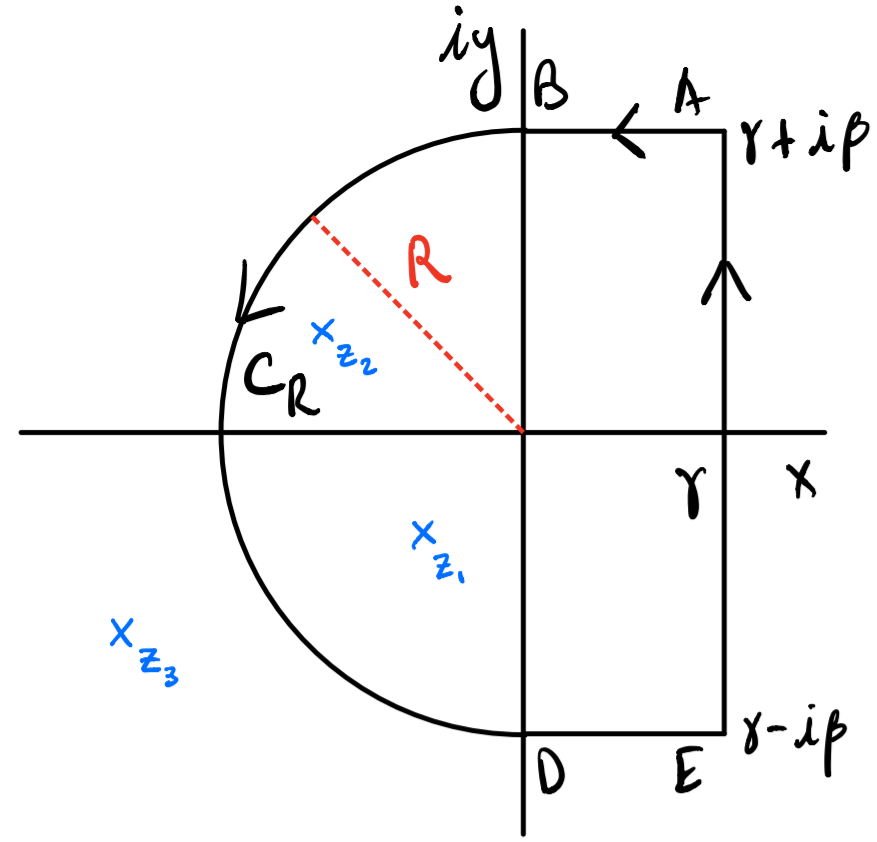
\includegraphics[scale=0.25]{3}
      \end{figure}
    \end{columns}

  All three of the extraneous contours vanish as we take $\beta$ (or $R$) to be arbitrarily large.

\end{frame}

\begin{frame}
  \frametitle{results of contour surgery}

  Hence the inversion integral can be computed by just summing up the residues of $e^{zt}f(z)$ at each isolated singularity to the left of the line on which the integral is taken. \[F(t) = \frac{1}{2\pi i}\int_{\gamma-i\infty}^{\gamma+i\infty} e^{zt}f(z)\dd{z} = \sum_k \Res(e^{zt}f(z), z_k)\]

\end{frame}

\section{a cute example}

\begin{frame}
  \frametitle{compute the inverse transform of $\br{s^2+1}^{-1}$}

  (it is $\sin(t)$)\vspace{7cm}

\end{frame}

\begin{frame}
  \frametitle{extra slide in case I had comments}

  

\end{frame}

\end{document}